\section{TreeKEM security} \label{sec:treekem-security}

\subsection{Commits with proposals in TreeKEM} \label{sec:treekem-overview-proposals}

In order to motivate our definitions for the syntax and security of CGKA schemes, we will first finish our discussion of the TreeKEM protocol from Section~\ref{sec:treekem-overview}.

\paragraph{Remove and update proposals} Recall the example of a commit without proposals in Section~\ref{sec:simple-commit}. Things look a bit different if the commit contains a remove proposal. Say user $A$ creates a commit that contains a remove proposal for user $E$. We could just let $A$ replace the nodes on $E$'s direct path $E$ and not encrypt anything for $E$. However, if $A$ were compromised while replacing $E$'s direct path and performed another commit to update their key material after the compromise, the information leaked in the compromise could still be used to compute the new group key, as it includes the secret keys of the nodes on $E$'s direct path.
Instead, $E$'s leaf and all nodes on $E$'s direct path are replaced by \emph{blank} nodes: nodes with no associated key pair. Now $A$ has to encrypt the secret $s_3$ directly to $F$ and to the parent node of $G$ and $H$ in the commit removing user $E$. See Figure~\ref{fig:treekem-remove}. A blank leaf node can be populated with a new user. A blank node that is not a leaf will be replaced by a non-blank node once some user in the node's subtree performs a commit. Blank nodes are also useful to represent the nodes of a subtree with no users.

\begin{figure}
	\begin{center}
		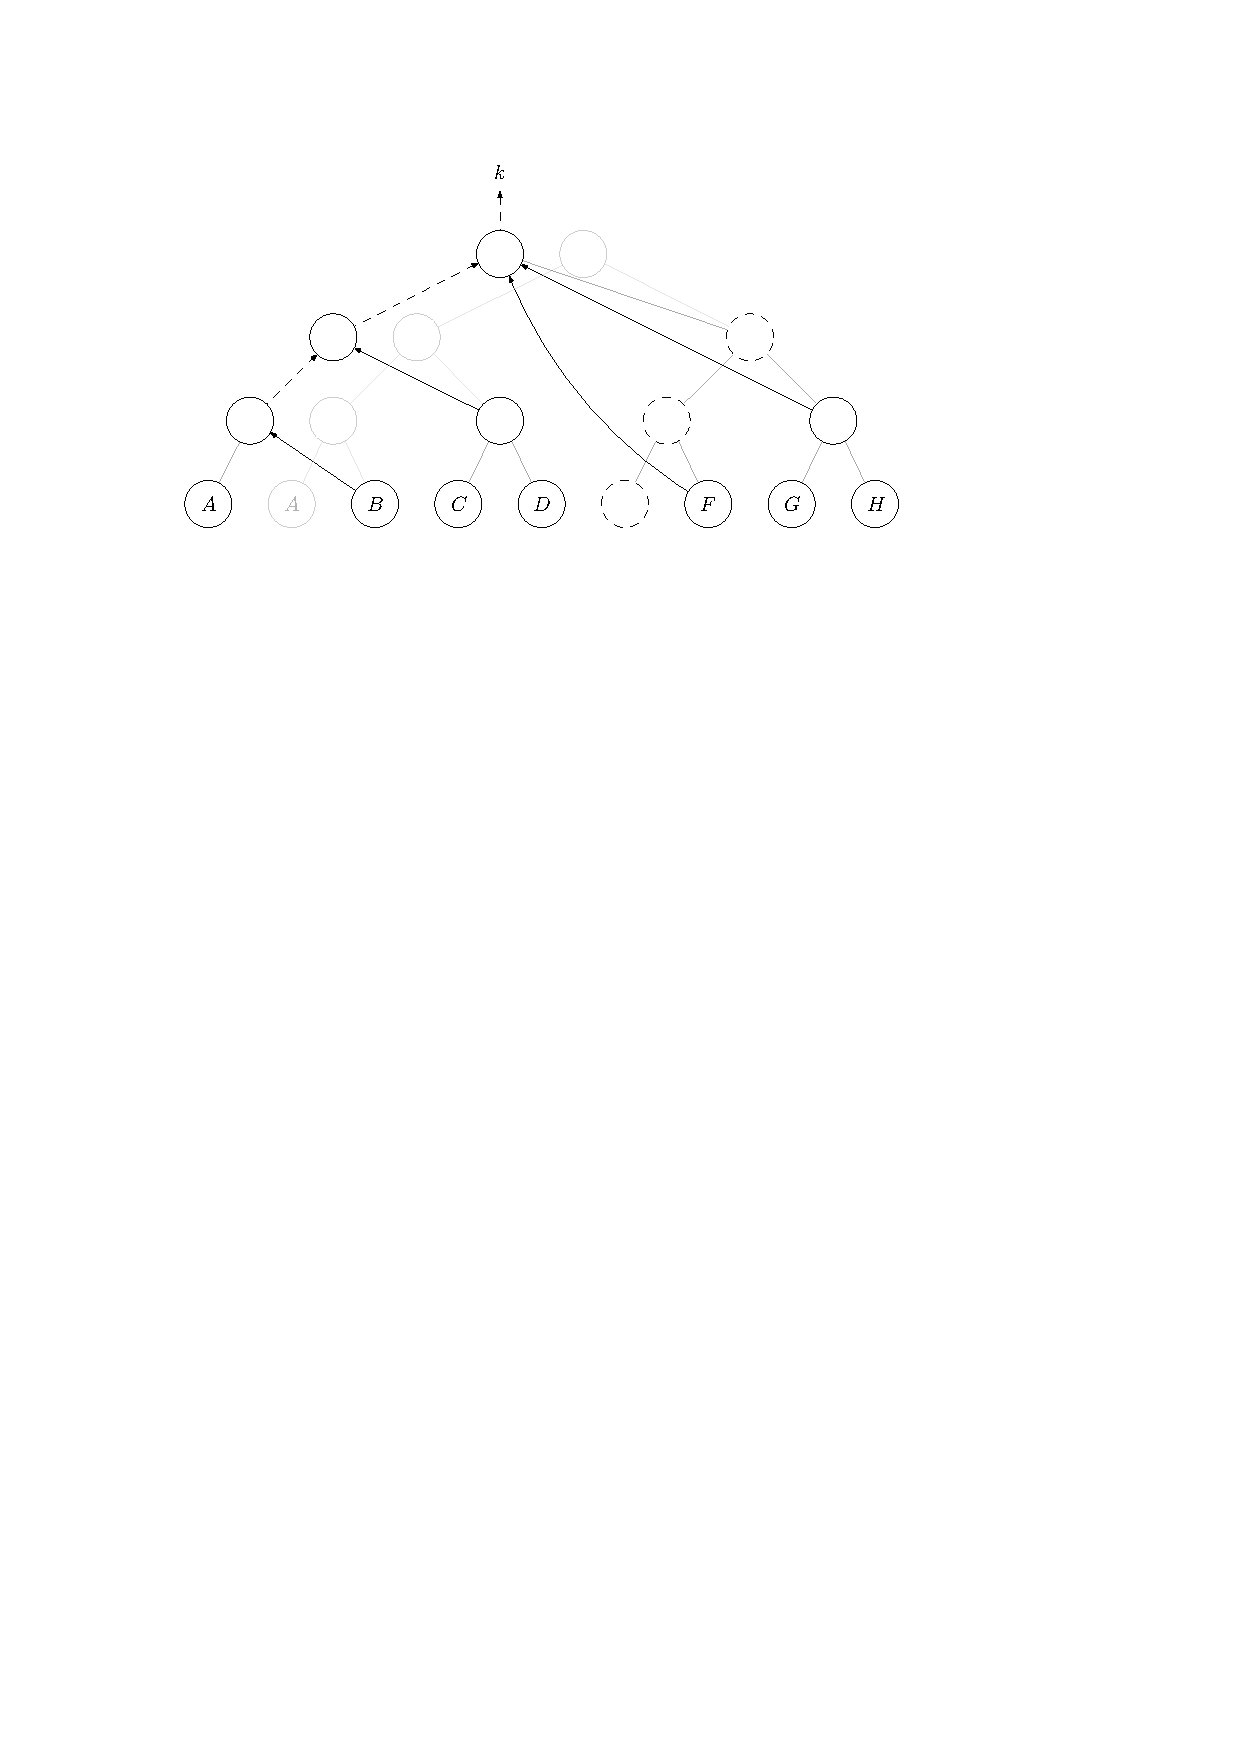
\includegraphics{figures/treekem-remove}
	\end{center}
	\caption{The commit by user $A$ removing user $E$ described in the text. Nodes with a dashed border represent the (new) blank nodes.}\label{fig:treekem-remove}
\end{figure}

Creating a commit with an update proposal for user a $u$ is analogous. The update proposal simply contains the public key of user $u$'s new leaf, while $u$ stored the corresponding secret key locally when creating the proposal. Because we don't want the committer to know the secret keys along $u$'s direct path, we must again replace these nodes with blank ones and encrypt to the non-blank nodes below directly.

\paragraph{Add proposals} Adding a user introduces one new but similar complication. Consider the same group as in Figure~\ref{fig:treekem-tree}, but with the leaf of user $H$ blank. Now say user $A$ would like to add user $H$ to the group. Although we would want $H$ to know all secret keys on their direct path, $A$ can only provide the secrets of their lowest common ancestor, which is the root node in this case.
In such a situation where a non-blank node $n$ has a leaf $l$ below it where $l$ does not know $n$'s secret key, we say that $l$ is \emph{unmerged} relative to $n$. Every non-blank, non-leaf node stores its list of unmerged leaves and whenever one encrypts to a node, one should also encrypt to all its unmerged leaves. A user's leaf becomes ``merged'' as the nodes on their direct path are replaced and they are provided the seeds to compute the secret keys of the new nodes.
Note that for any non-leaf node $n$, any one of its descendants $d$ and any unmerged leaf of $n$ that is a descendant of $d$, this leaf must also be an unmerged leaf of $d$: every commit that replaces $d$ also replaces the node $n$ and if a user at a leaf learns the secret key of the new node for $d$ through its seed, they also learn the seed of and therefore the secret key of the new node for $n$. Figure~\ref{fig:treekem-add} shows a commit by user $A$ adding $H$, followed by another commit by user $E$.

\begin{figure}
	\centering
	\begin{subfigure}[b]{\textwidth}
		\centering
		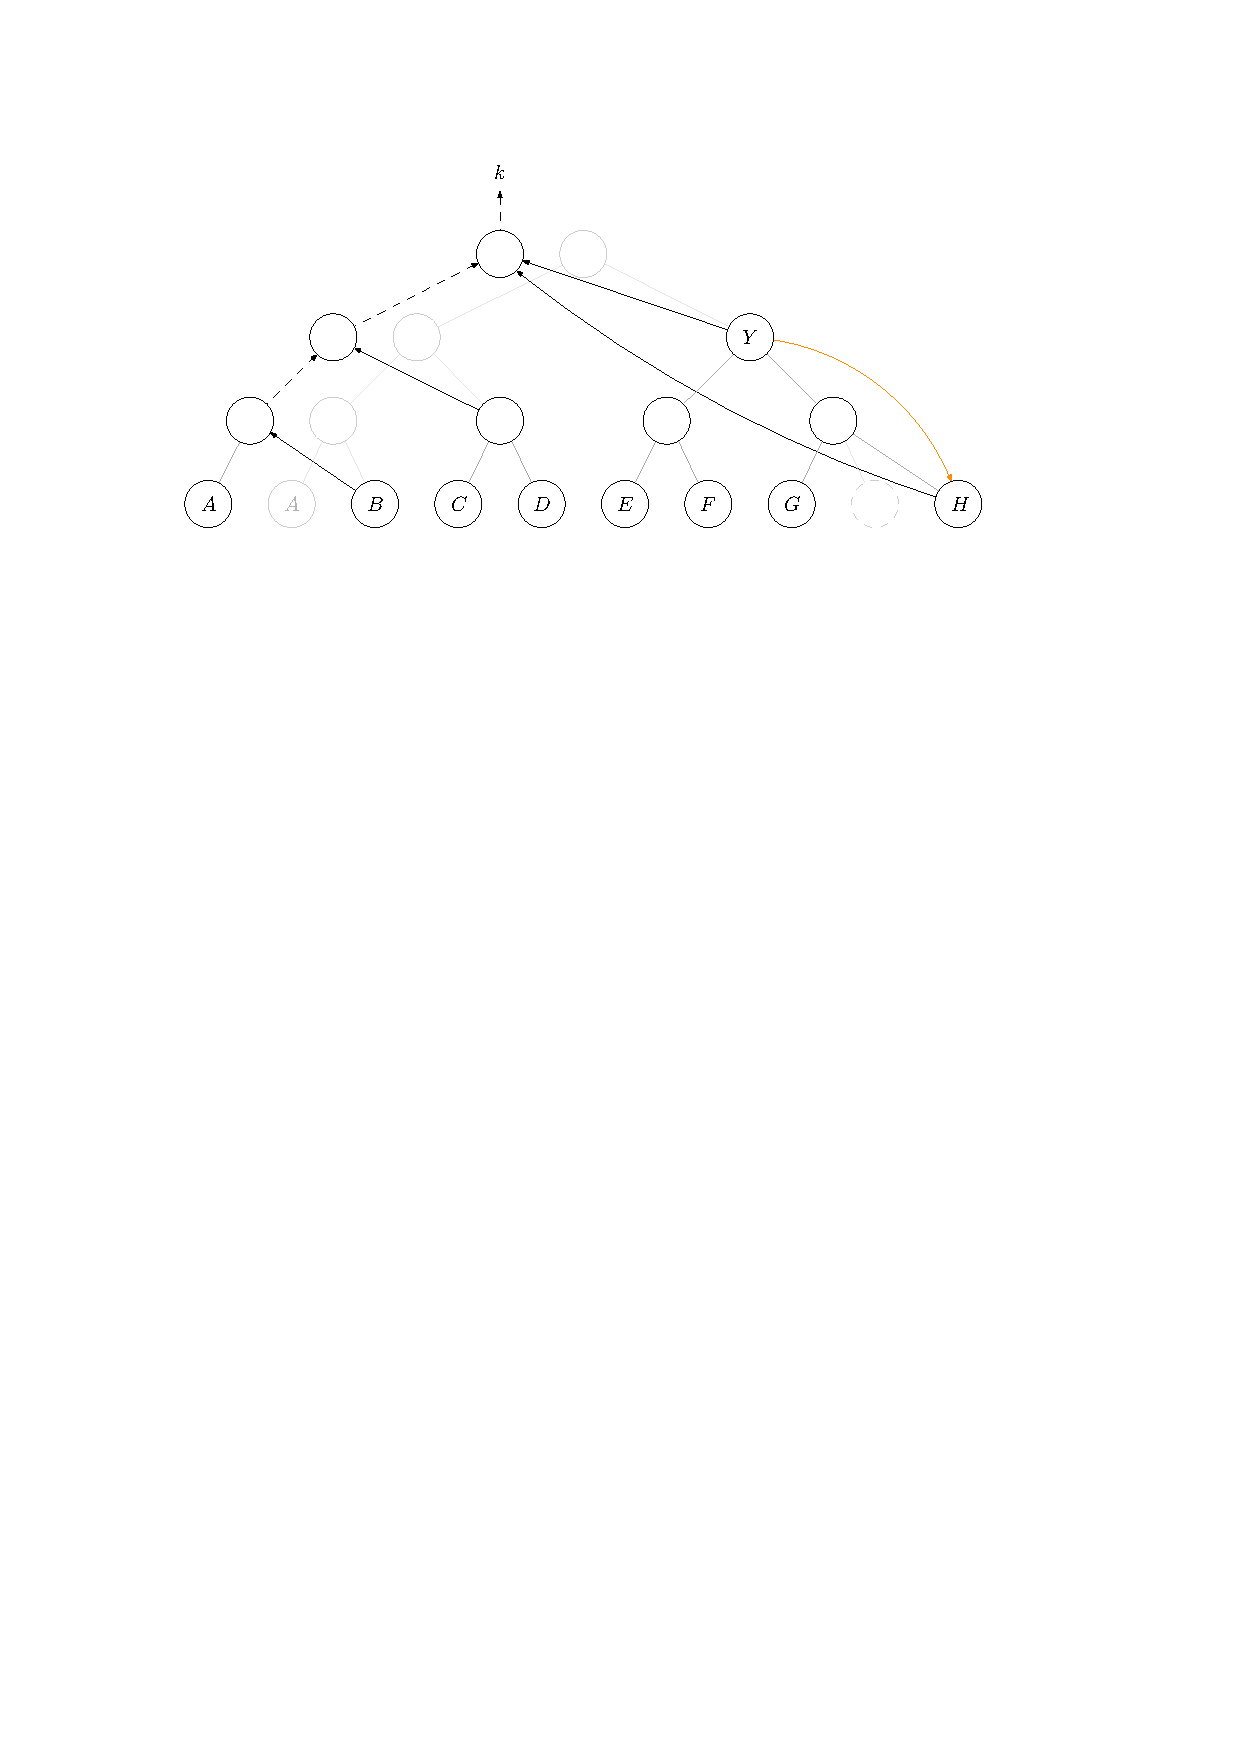
\includegraphics[width=\textwidth]{figures/treekem-add-1}
		\caption{User $A$ adds user $H$. As a small detail: the encryption for user $H$ is computed using $H$'s init key instead of the public key of their leaf.}
		\label{fig:treekem-A-add-H}
	\end{subfigure}
	\begin{subfigure}[b]{\textwidth}
		\centering
		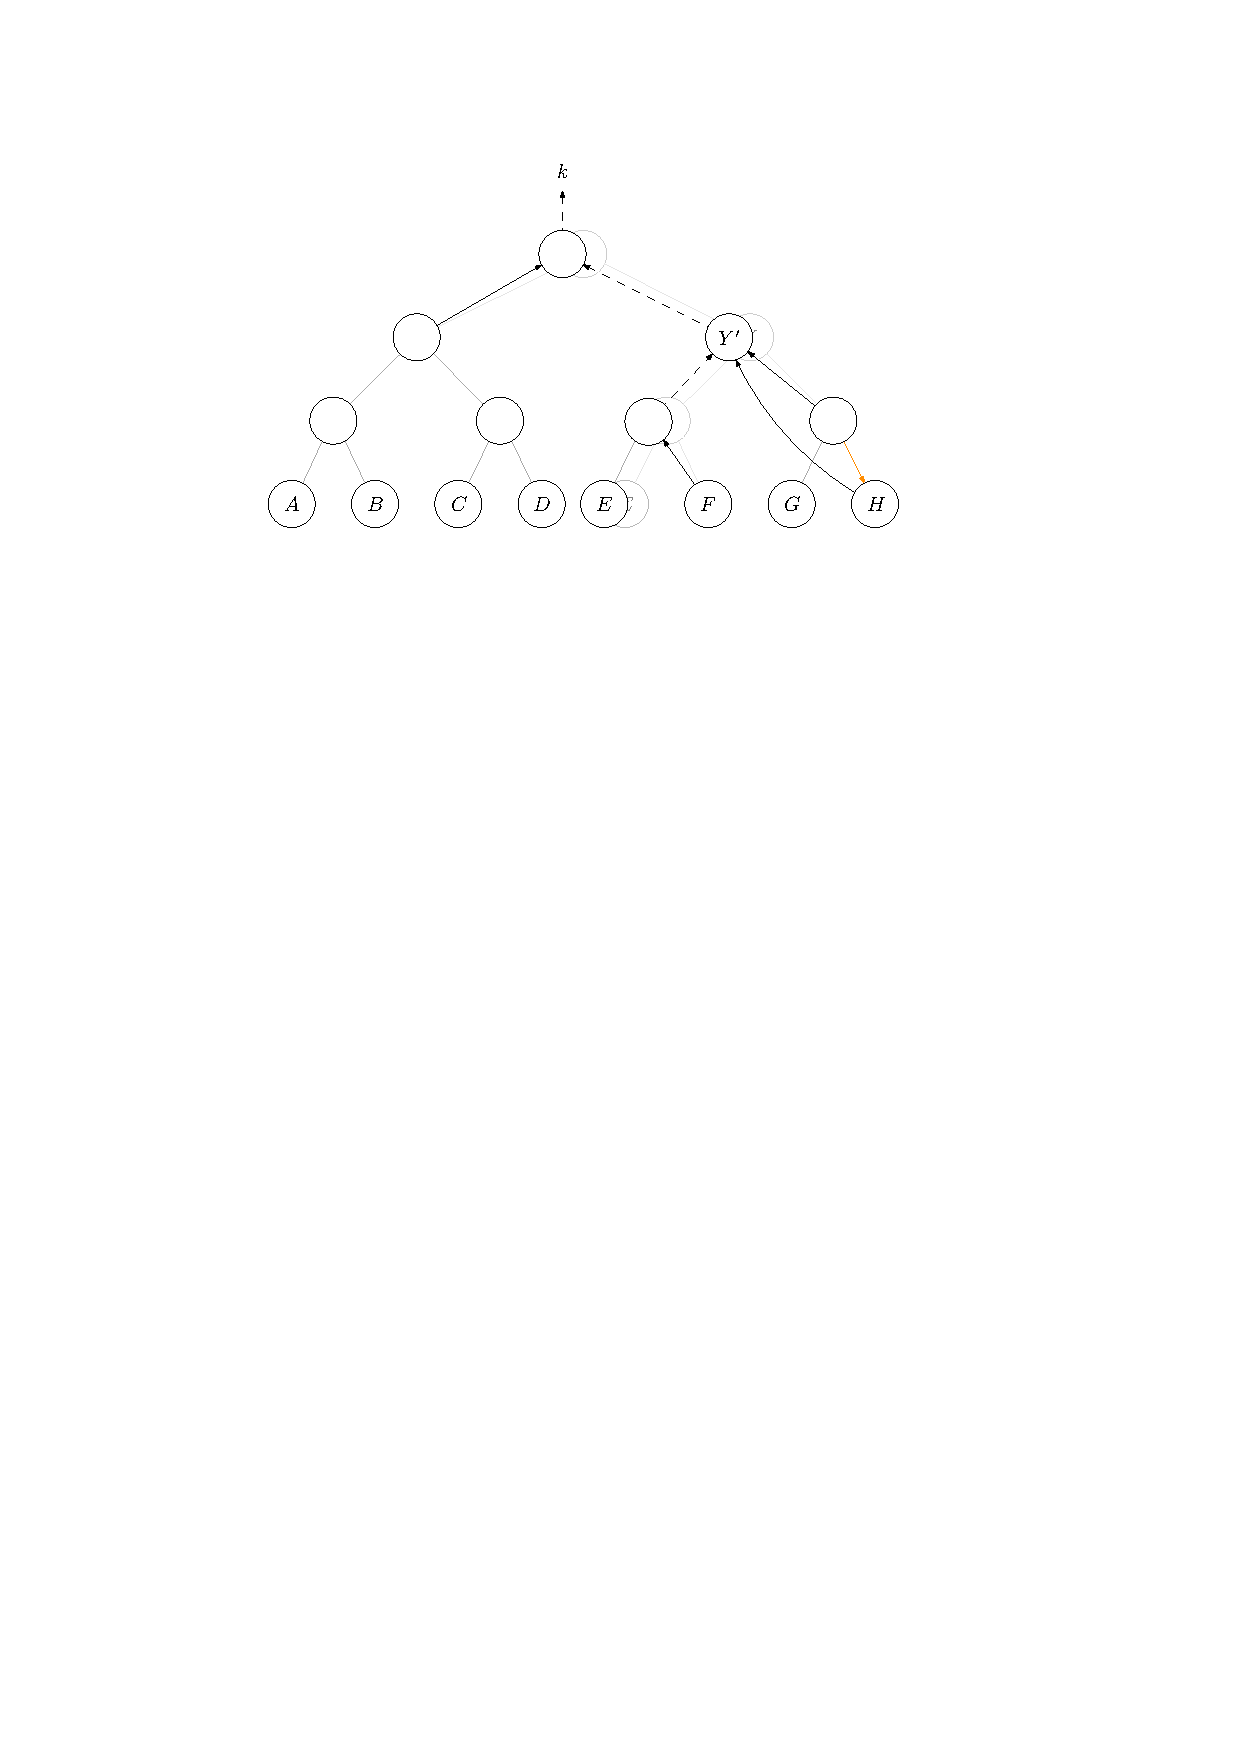
\includegraphics[width=\textwidth]{figures/treekem-add-2}
		\caption{Commit by user $E$. $H$ is now ``merged'' relative to node $Y'$.}
	\end{subfigure}
	\caption{A commit adding user $H$ and another commit by a user $E$ as described in the text. Orange edges illustrate the fact that the target leaf is unmerged relative to the source node. In \subref{fig:treekem-A-add-H}, $H$ is also unmerged relative to $Y$'s right child, but this information is redundant as it follows from $H$ being unmerged relative to $Y$.}
	\label{fig:treekem-add}
\end{figure}

\paragraph{Resolution} We have now seen that when performing a commit, one must pay attention to blank nodes and unmerged leaves when providing encryptions. Instead of only providing encryptions for each node on the copath as in the ideal case, in the general case for each node $n$ on the copath one must provide an encryption for every node in the \emph{resolution} of $n$. The resolution of a non-blank node is the node itself and the set of all its unmerged leaves. The resolution of a blank leaf is the empty set and the resolution of a blank, non-leaf node is the union of the resolutions of its two children.

\paragraph{Key packages and welcome messages} To encrypt to an existing group member it is clear that we can just use the public key in their leaf. But how do we encrypt to a new user? Before a user joins any group, they publish a \emph{key package}: this contains (among other things) the public key, their so-called \emph{init key}, to be used to encrypt information to the user when they join the group and the public key that should be associated with the user's leaf. The key package is included (or referenced) in the add proposal for the new user. Along with the seed of the committer's and the new user's lowest common ancestor in the tree, the new user must also be given the (public) state of the tree. This information is provided to the new user, encrypted with their init key, by the committer in a \emph{welcome message}.

\subsection{Continuous Group Key Agreement}

\subsubsection{The model}

As already described briefly in the introduction, a CGKA scheme allows a group of users to agree on a group key, indistinguishable from random for any eavesdropper, while providing mechanisms to add or remove users from the group and update the group key and users' key material, such that FS and PCS can be achieved.

Fully modelling a group of users running a CGKA scheme is complex. Since the protocol must work in the asynchronous setting, there must be a delivery service that takes protocol messages and forwards them to the recipients. Users also need to be able to publish some kind of public key, the key packages used in TreeKEM, such that they can be invited to the group with a welcome message. This functionality is also left to the delivery service. Moreover, there must be mechanisms in place to authenticate protocol messages and the published public keys.

In our model, users are honest nodes running the protocol algorithms and maintaining local state. They send out new messages and process received messages immediately. They have a reliable communication channel to the delivery service, and all public keys and protocol messages are assumed to be authenticated, meaning that an attacker cannot forge them. The delivery service, and thus an attacker, can of course see all protocol messages. We assume little about what messages get delivered by the delivery service: the service may deliver a message to some users but not others and it may not deliver certain messages at all.

For a more complete model we refer the reader to \cite{modular-group-messaging}. The authors consider not just CGKA but the more difficult problem of \emph{secure group messaging} as tackled by the MLS protocol. The model they consider allows an attacker to inject protocol messages and gives them some control over the public keys stored by the delivery service.

\subsubsection{PC-CGKA schemes}

Multiple definitions of the syntax and security of CGKA schemes already exist \cite{rtreekem,ttkem,modular-group-messaging}, all meant to capture the syntax of how update, add and remove operations were performed with the latest verion of TreeKEM at the time, and all with the same name. As already described in the introduction, the current version of TreeKEM uses propose and commit operations to advance the group state, which is also the syntax formalized in \cite{modular-group-messaging} and in this work. The syntax defined in \cite{rtreekem,ttkem} came before the propose and commit syntax was introduced. In this syntax there are no proposals and every operation is a commit, either adding a single user, removing a single group member, or just updating the key material of the committer. To differentiate our definitions from existing ones that describe something different as in \cite{rtreekem,ttkem}, we will talk about \emph{propose and commit continuous group key agreement} (PC-CGKA) schemes.

\paragraph{Syntax}

Our definition of the syntax of PC-CGKA schemes is inspired from the definition in \cite{ttkem} and is essentially the same as what is described in \cite[Section 4.1.1]{modular-group-messaging}. We assume that every user $u$ is identified by some value $id_u$.

\begin{definition}[PC-CGKA]
	Let $\eta$ denote the security parameter.
	A \emph{PC-CGKA scheme} $\Sigma$ with key space $\mathcal{K}$ consists of the following algorithms:
	\begin{enumerate}[1.]
		\item[] \textsc{Initialization:}
			\begin{itemize}
				\item An algorithm $\gen$. Before joining any group, a user generates a pair of keys $(pk, sk) \from \gen(1^\eta)$, a public and private key.
				\item An algorithm $\operatorname{CreateGroup}$. A user runs $\sigma \from \operatorname{CreateGroup}(1^\eta)$ to locally initialize a group with themselves as the only member and the state of the group stored in $\sigma$. We call $\sigma$ their \emph{group state}.
			\end{itemize}
		\item[] \textsc{Compute the group key:}
			\begin{itemize}
				\item An algorithm $\operatorname{Key}$. At any point in time, a member of a group with state $\sigma$ can compute the current \emph{group key} $k \from \operatorname{Key}(\sigma)$ with $k \in \mathcal{K}(\eta)$.
			\end{itemize}
		\item[] \textsc{Proposal:}
			\begin{itemize}
				\item An algorithm $\operatorname{ProposeUpdate}$. If a member $u$ of a group with state $\sigma$ wishes to update their key material, they may run $(\sigma, p) \from \operatorname{ProposeUpdate}(\sigma)$ to create an \emph{update proposal} $p$ to be shared with other members of the group and update their state such that they have processed $p$.
				\item An algorithm $\operatorname{ProposeAdd}$. If a member of a group with state $\sigma$ wishes to add a new user $u$ with public key $pk_u$ to the group, they may run $(\sigma, p) \from \operatorname{ProposeAdd}(\sigma, id_u, pk_u)$ to create an \emph{add proposal} $p$ to be shared with other members of the group and update their state such that they have processed $p$.
				\item An algorithm $\operatorname{ProposeRemove}$. If a member of a group with state $\sigma$ wishes to remove another member $u$ from the group, they may run $(\sigma, p) \from \operatorname{ProposeAdd}(\sigma, id_u)$ to create a \emph{remove proposal} $p$ to be shared with other members of the group and update their state such that they have processed $p$.
			\end{itemize}
		\item[] \textsc{Commit:}
			\begin{itemize}
				\item An algorithm $\operatorname{CreateCommit}$. To apply a list of proposals $\pi$ to the group state, a member with state $\sigma$ may run $(\sigma', c, w_{_1}, \ldots, w_{_k}) \from \operatorname{CreateCommit}(\sigma, \pi)$, where $c$ is a \emph{commit} to be shared with other members, $\sigma'$ would be the new state of the member after applying the commit\footnote{Note that the user's state is not immediately replaced with the new state output by the algorithm. We will see why in the explanation of the semantics below.} and each $w_{i}$ is a \emph{welcome message} for a newly added user.
			\end{itemize}
		\item[] \textsc{Process:}
			\begin{itemize}
				\item An algorithm $\operatorname{ProcessCommit}$. Upon receiving another member's commit $c$, a member $u$ with state $\sigma$ can set $\sigma \from \operatorname{ProcessCommit}(\sigma, c)$ to process $c$. We say that $u$ has \emph{processed} $c$.
				\item An algorithm $\operatorname{ProcessWelcome}$. Upon receving a welcome message $w$ for a user with public key $pk$, the user with this public key can set $\sigma \from \operatorname{ProcessWelcome}(pk, sk, w)$, where $sk$ is the corresponding secret key output by $\gen$.
			\end{itemize}
	\end{enumerate}

	For any object $X$ above (including $\mathcal{K}$) we will refer to it as $\Sigma.X$.

	The scheme must also specify an algorithm for determining the set of members of the group from a group state $\sigma$.
\end{definition}

\paragraph{Semantics} In the following we provide some further details regarding the semantics of the PC-CGKA algorithms:
\begin{itemize}
	\item $\gen$: The public key is used to invite the user to the group and should therefore be made public. This public key corresponds to a key package in TreeKEM (see Section~\ref{sec:treekem-overview}). The same key pair must not be reused to join multiple groups and must be discarded after it was used to join a group. A new key pair must be generated to join a new group.
	\item $\operatorname{ProposeUpdate}$: An update proposal created by a user $u$ contains (possibly public) information for the other group members about $u$'s new key material. This information is used by other members to provide encrypted information in a commit (see below) that includes the update proposal such that $u$ is able to compute the new group key.
	\item $\operatorname{CreateCommit}$: Let $c$ a commit and $w_1, \ldots, w_k$ the corresponding welcome messages output by the algorithm, run by user $u$ with group state $\sigma$ and with the proposals $\pi$ provided as input. There should be one welcome message for each new user added to the group in the commit with a corresponding add proposal in $\pi$. Welcome message $w_i$ contains the identifier $id_i$ of a user and the message should be shared with that user such that they can join the group. Besides updating the key material for all other members with an update proposal in $\pi$, the commit also updates user $u$'s key material. Accordingly, $\pi$ should not contain an update proposal for user $u$. Nor should it contain a remove proposal for user $u$ as they will know the group key resulting from the commit. User $u$ may keep both group states $\sigma$ and $\sigma'$ until the group agrees on whether to apply the commit $c$ or not. If the commit is to be applied, user $u$ sets their state to $\sigma'$ and discards $\sigma$. Otherwise, they discard $\sigma'$. Applying a commit results in a new group key.

	      Our syntax does not specify how a user learns of proposals in $\pi$ created by other users. Also how users agree on whether to apply a commit is left up to the application. The decision could be made by the delivery service or using some consensus algorithm run by all group members.

	      We see a call to $\operatorname{CreateGroup}$ as a special type of commit that is applied by the group creator.


	\item $\operatorname{ProcessCommit}$: If the commit removed the member from the group, they should not be able to compute the group key from $\sigma$ and should delete $\sigma$.
	\item $\operatorname{ProcessWelcome}$:  The user must discard their secret key $sk$ after processing a welcome message, so that the contents of the welcome message remain secret in case the user gets compromised (recall FS). As we cannot express this conveniently with our syntax, our security definition does not check for this (and does not give the adversary the secret key if a user is compromised after having processed their welcome message).
\end{itemize}

\paragraph{Correctness}

The above description of semantics already provides some explicit correctness properties or implicitly implies other ones. We will explicitly define one important correctness property that a PC-CGKA scheme should satisfy in Definition~\vref{def:cgka-correctness-consistent-history}. \todo{Justify why I mention this property and why it is important. Explain examples of commit history and why it plays a role in security.}

The correctness property concerns the handling of ``bad'' (malformed or inconsistent) inputs. The algorithms of a PC-CGKA scheme should have several checks built in to deal with such inputs. For example
\begin{itemize}
	\item a commit including an update or add proposal for the commit creator is invalid
	\item a user should never process the same commit twice
	\item a user should never process a commit that they created
	\item etc.
\end{itemize}
Many of these checks are straightforward and we do not provide an extensive list of what is needed. However, we will discuss one type of check that is less straightforward and plays a role in the security of the scheme. Our correctness property enforces all members of a group to agree on the history of commits they have applied (up to joining the group). It avoids scenarios where a group member may skip a commit processed by other members that, for example, removed a user from the group. We ignore errors that would result from processing bad input in our syntax and restrict our security model to dealing with only valid inputs, as it is not our goal to analyze this type of attack on the scheme.

Before we can formally define our correctness property, we must first introduce some definitions.

\begin{definition}[Applying a commit]
	When a user
	\begin{itemize}
		\item processes commit $c$ with $\operatorname{ProcessCommit}$
		\item creates commit $c$ and subsequently updates their group state to the new state output by the corresponding call to $\operatorname{CreateCommit}$
		\item joins the group by processing welcome message $w$, where $c$ is the commit that was output along with $w$ by $\operatorname{CreateCommit}$
		\item creates a group, where we let $c$ denote the call to $\operatorname{CreateGroup}$
	\end{itemize}
	we say that the user \emph{applied} commit $c$.
\end{definition}

In the following, when talking about \emph{time} for a user that was a part of some group, we are referring to the sequence of group states they went through as members of the group\footnote{We are only interested in state transitions from applying a commit, but for completeness we will also consider transitions due to creating proposals as a part of this sequence.}.

\begin{definition}[Last commit]
	Let $u$ a user that at some point in time was a member of a group and had group state $\sigma$. We define the \emph{last commit} in $\sigma$ to be the most recent commit $c$ that $u$ applied up to arriving in state $\sigma$.
\end{definition}

In the above definition, the user's last commit will always exist since they either joined the group through a welcome message or created the group themselves.

\begin{definition}[Consistent group states] \label{def:consistent-group-state}
	Let $u_0, u_1$ two users where each user was a member of a group at some point in time. Let $\sigma_0, \sigma_1$ the group states they were in, respectively and $c_0, c_1$ the last commits in $\sigma_0, \sigma_1$, respectively. The group states $\sigma_0$ and $\sigma_1$ are said to be \emph{consistent} if $c_0 = c_1$.\footnote{If a commit is a call to $\operatorname{CreateGroup}$, it is equal to another commit iff.\ both refer to the same call to $\operatorname{CreateGroup}$. This implies that after a user just created a group, their group state is consistent with itself only.}
\end{definition}

We can now define the correctness property motivated above.

\begin{definition}[Consistent history] \label{def:cgka-correctness-consistent-history}
	A PC-CGKA scheme $\Sigma$ \emph{maintains a consistent hisory} if a user with group state $\sigma$ only successfully\footnote{As noted, we ignore checks for bad input in our syntax. To describe schemes satisfying correctness related to bad inputs, one would need to extend the syntax such that e.g.\ an algorithm can also output an error, and the user's state remains unchanged if this is the case.} processes a commit $c \from \operatorname{CreateCommit}(\sigma', \cdot)$ for some $\sigma'$\footnote{Here we only consider states $\sigma'$ that an honest user would get as output from one of the PC-CGKA algorithms.} (with $\operatorname{ProcessCommit}$) if $\sigma$ and $\sigma'$ are consistent.
\end{definition}

Definition~\ref{def:consistent-group-state} also allows us to express the following important correctness property: any set of members with consistent group states must compute the same group key with $\Sigma.\operatorname{Key}$ and must agree on the set of members of the group.

In the following we introduce a few more definitions that will become useful later.

\begin{definition}[Parent commit]
	Let $c$ a commit output by $\operatorname{CreateCommit}(\sigma_0, \cdot)$ for some $\sigma_0$. The \emph{parent commit} of $c$ is the last commit in $\sigma_0$.
\end{definition}

Note that if the PC-CGKA scheme maintains a consistent history, for a commit $c$ that was processed by a user while they were still in group state $\sigma$, the last commit in $\sigma$ will be the parent commit of $c$.

\begin{definition}[Commit history] \label{def:commit-history}
	Let $c$ a commit.\footnote{Here we only consider commits referring to a call to $\operatorname{CreateGroup}$ or output by $\operatorname{CreateCommit}$, run by an honest user.} Define the \emph{commit history} of $c$ as follows:
	\begin{itemize}
		\item \textbf{Case $c$ refers to a call to $\operatorname{CreateGroup}$:} the sequence $(c)$ of length 1
		\item \textbf{Otherwise:} the sequence $(c_1, \ldots, c_k, c)$, where $(c_1, \ldots, c_k)$ is the commit history of $c$'s parent commit $c_k$.
	\end{itemize}
\end{definition}

One could also consider the \emph{local} commit history of a group member $u$ in group state $\sigma$, consisting of the sequence of commits applied by $u$ since joining the group and until arriving in $\sigma$. If the PC-CGKA scheme maintains a consistent history, this local commit history is a suffix of the commit history of the last commit in $\sigma$. (To see this, first note that by definition the last commit in $\sigma$ is the last commit the local commit history. Then repeatedly apply the argument before Definition~\ref{def:commit-history}.) Thus, for a set of users in consistent group states, the users all agree on the commits they have processed and their order (up to the earliest commit present in the local commit history of all users).

\subsubsection{PC-CGKA security}

Our security definition is again inspired by \cite{ttkem}. We consider fully adaptive adversaries. The adversary controls all PC-CGKA operations performed by the users, can decide who receives what messages (i.e.\ the adversary has control over the delivery service), can decide what commits get applied or discarded, and when they are discarded, by querying ``$\operatorname{confirm}$'' and can corrupt the state of any user. We will refer to commits created by a user that they have not yet been told to apply or discard as \emph{unconfirmed commits}. Corrupting a user leaks the group states corresponding to all their unconfirmed commits. Because the adversary can schedule the delivery of messages as it likes, it is possible for the adversary to create ``forks'' in the group where some users in the group are told to process one commit, while other users are told to process another. Such forks could also happen in practice and should not break security.

The adversary eventually chooses a commit to be challenged on, for which they must differentiate the group key from a uniformly random key. We must restrict the set of commits the adversary can ask to be challenged on to those that are expected to be \emph{safe} even in the face of previous or later corruptions. The level of FS and PCS expected from a PC-CGKA scheme is captured by the size of this set of safe commits. Exactly which commits are considered safe will be explained later.

We also impose some notable restrictions on the adversary. The adversary cannot inject protocol messages or public keys and it may only deliver a message to users that are supposed to process that message, in order to avoid giving users messages with bad inputs. The latter restriction is justified, as in a correct PC-CGKA protocol such messages would simply be discarded and correctness can be verified independently. Imposing the restriction on the adversary allows us to ignore the details of handling bad inputs when specifying a PC-CGKA scheme and to analyze the core aspects of its security.

The definition in \cite[Section B.1]{modular-group-messaging} is very similar in essence. The same restricions on the adversary are imposed. However, the security game provided there gives more power to the adversary: the adversary may additionally choose the randomness used in operations, choose its own public keys to be associated with users and tell certain users not to delete old keys. In the end this restricts the set of safe commits. We provide our own definition with the hope of having a formulation that is easier to digest, keeps the security game simpler and is more explicit about what commits are considered safe.

\begin{definition}[The PC-CGKA game]
	Let $\Sigma$ a PC-CGKA scheme. Define the game $\game{\Sigma}{\eta}{PC-CGKA}(\adv)$ for an adversary $\adv$:
	\begin{enumerate}[1.]
		\item \label{def:cgka-game-step-init} $\adv$ outputs $n \in \mathbb{N}$. For each $i \in [n]$, initialize a user $i$ by creating a (unique) identifier $id_i$, generating $(pk_i, sk_i) \from \Sigma.\gen(1^\eta)$, preparing $U_i = \varnothing$, the set of unconfirmed commits at user $i$, and setting $\sigma_i \coloneqq \varnothing$, where $\varnothing$ denotes the empty value. The state output by an algorithm of $\Sigma$ is never the empty value. $\adv$ is given $(pk_1, id_1), \ldots, (pk_n, id_n)$.

		      Set $P = C = W = 0$, where $P$ denotes the number of proposals, $C$ the number of commits and $W$ the number of welcome messages created.
		\item $\adv$ may adaptively do the following queries:
		      \begin{itemize}
			      \item $\operatorname{create-group}(i)$ for $i \in [n]$: set $\sigma_i \from \operatorname{CreateGroup}(1^\eta)$.
			      \item $\operatorname{propose-update}(i)$ for $i \in [n], \sigma_i \neq \varnothing$: run $(\sigma_i, p_{P + 1}) \from \operatorname{ProposeUpdate}(\sigma_i)$ to update user $i$'s state and get a proposal $p_{P + 1}$. $\adv$ is given $p_{P + 1}$. Set $P \coloneqq P + 1$.
			      \item $\operatorname{propose-add}(i, j)$ for $i, j \in [n], \sigma_i \neq \varnothing$: run $(\sigma_i, p_{P + 1}) \from \operatorname{ProposeAdd}(\sigma_i, id_j, pk_j)$ to update user $i$'s state and get a proposal $p_{P + 1}$. $\adv$ is given $p_{P + 1}$. Set $P \coloneqq P + 1$.
			      \item $\operatorname{propose-remove}(i, j)$ for $i, j \in [n], \sigma_i \neq \varnothing$: run $(\sigma_i, p_{P + 1}) \from \operatorname{ProposeRemove}(\sigma_i, id_j)$ to update user $i$'s state and get a proposal $p_{P + 1}$. $\adv$ is given $p_{P + 1}$. Set $P \coloneqq P + 1$.
			      \item $\operatorname{create-commit}(i, (j_1, \ldots, j_d))$ for $i \in [n], \sigma_i \neq \varnothing, \forall l \; j_l \in [P]$: run $(\sigma, c_{C + 1}, w_{W + 1}, \ldots, w_{W + k}) \from \operatorname{CreateCommit}(\sigma_i, (p_{j_1}, \ldots, p_{j_d}))$ to create the new state $\sigma$, commit $c_{C + 1}$ and corresponding welcome messages. $\adv$ is given $c_{C + 1}$ and $w_{W + 1}, \ldots, w_{W + k}$. Set $U_i \coloneqq U_i \cup \{(C + 1, \sigma)\}$, $C \coloneqq C + 1$ and $W \coloneqq W + k$.
			      \item $\operatorname{confirm}(j, b)$ for $j$ s.t.~$(j, \sigma) \in U_i$ for some user $i$ and state $\sigma$, $b \in \{0, 1\}$: If $b = 0$, set $U_i \coloneqq U_i \setminus \{(j, \sigma)\}$. If $b = 1$, set $\sigma_i \coloneqq \sigma$ and $U_i \coloneqq \varnothing$.\footnote{All other unconfirmed commits in $U_i$ are cleared if $b = 1$ as they should not be applied anymore.}
			      \item $\operatorname{deliver-commit}(i, j)$ for $i \in [n], \sigma_i \neq \varnothing, j \in [C]$: run $\sigma \from \operatorname{ProcessCommit}(\sigma_i, c_j)$. Set $U_i \coloneqq \varnothing$. If $c_j$ contains a remove proposal for user $i$, then set $\sigma_i \coloneqq \varnothing$, generate a new pair $(pk_i, sk_i) \from \Sigma.\gen(1^\eta)$ and give $(i, pk_i)$ to $\adv$. Otherwise, set $\sigma_i \coloneqq \sigma$.
			      \item $\operatorname{deliver-welcome}(i, j)$ for $i \in [n], \sigma_i = \varnothing, j \in [W]$: set $\sigma_i \from \operatorname{ProcessWelcome}(pk_j, sk_j, w_j)$.\footnote{Note that in a real execution of the protocol the user must delete $sk_j$ from their local state after processing the welcome message $w_j$. Accordingly, $sk_j$ is no longer leaked to the adversary in a later query $\operatorname{corrupt}(j)$.}
			      \item $\operatorname{corrupt}(i)$ for $i \in [n]$: If $\sigma_i = \varnothing$, $\adv$ is given $sk_i$. Otherwise, $\adv$ is given $\sigma_i$ and $U_i$.
		      \end{itemize}
		\item $\adv$ picks $i \in [0, C]$. We call the commit $c_i$ the \emph{challenge commit}, where $c_0$ refers to the initial $\operatorname{CreateGroup}$ operation. Let $\sigma$ the group state output by the operation that created $c_i$ (the state output by $\operatorname{CreateCommit}$ if $i > 0$ or the state output by $\operatorname{CreateGroup}$ if $i = 0$). A bit $b \from \{0, 1\}$ is sampled and $\adv$ is given
		      \[
			      k = \begin{cases}
				      \Sigma.\operatorname{Key}(\sigma) & b = 0 \\
				      \tilde{k}                         & b = 1
			      \end{cases},
		      \]
		      where $\tilde{k} \from \Sigma.\mathcal{K}(\eta)$. $\adv$ may continue to do queries as before.
		\item $\adv$ outputs a bit $b'$. The output of the game is defined to be $1$ if $b' = b$, and $0$ otherwise.
	\end{enumerate}

	We require an adversary playing the above game to adhere to the following:
	\begin{itemize}
		\item $\operatorname{create-group}$ is queried exactly once
		\item The challenge commit is safe (see Definition~\vref{def:safe-commit})
		\item For any query $\operatorname{deliver-commit}(i, j)$ where the commit $c_j$ was created by user $k$ while they where in state $\sigma_k'$, $\sigma_i$ and $\sigma_k'$ must be consistent
		\item For any query $\operatorname{create-commit}(i, (j_1, \ldots, j_d))$, for every proposal $p_{j_l}$ created by a user while in state $\sigma_l'$, $\sigma_i$ and $\sigma_l'$ must be consistent
		\item A user never processes a commit that they created
		\item Every commit is processed at most once by any user
		\item A welcome message for user $i$ is processed by $i$ at most once and is never processed by a user $j$ with $i \neq j$
		\item A user creating a commit never includes an update or remove proposal for themselves, or multiple update/add/remove proposals for to the same user
		\item A user is never asked to create an add proposal for a user they consider to be in the group, or create a remove proposal for a user they do not consider to be in the group
	\end{itemize}
\end{definition}

The concept of a safe user and safe commit is adapted from the so-called ``safe predicate'' in \cite{ttkem}, which again took inspiration from \cite{rtreekem}. As elaborated in the cited papers and also analogous to how we needed to define ``safe'' nodes in the SD-GSD game, we want to forbid the adversary to ask to be challenged on a commit for which it can trivially compute the group key through some corruption it performed.

To see what is needed for a commit to be safe, consider some commit $c$ with group key $k$ created by a user $i$ and let $j \neq i$ any user that $i$ would consider to be in the group after applying $c$ (Definition~\ref{def:group-members-after-applying-commit} clarifies exactly which users are considered to be in the group). The commit $c$ or an associated welcome message provides encrypted information for user $j$ to compute the new group key using its current key material. Clearly, if this key material has been compromised by the adversary corrupting user $j$, the commit should not be safe. If the adversary has not corrupted user $j$ since they last updated their key material, then we would not expect the adversary to be able to learn the group key $k$ through user $j$, even if user $j$ was corrupted before (recall PCS).
Moreover, corrupting user $j$ after they have again updated their key material should not allow the adversary to compute the group key of $c$ either (recall FS). We will later say that the commit $c$ is \emph{safe with respect to user $j$} if $j$ was not corrupted in this window between their last and next update.
Now, it is important to notice that the encrypted information in commit $c$ is for the key material that user $j$ had \emph{from user $i$'s view} when user $i$ created $c$. It is possible that when user $i$ created $c$, user $j$ had already processed a commit updating their key material that user $i$ has not yet processed. Thus, we must be careful to require exactly the right key material of user $j$ to be unknown to the adversary. Definition~\vref{def:safe-commit-wrt-user} formalizes this.

\begin{definition} \label{def:group-members-after-applying-commit}
	Let $c$ a commit and let $\sigma'$ the new group state ouptut by
	\begin{itemize}
		\item the call to $\operatorname{CreateCommit}$ that created $c$
		\item or the call to $\operatorname{CreateGroup}$ that $c$ refers to
	\end{itemize}
	The (set of) \emph{users in the group after applying $c$} is the set of users in the group according to state $\sigma'$.
\end{definition}


\begin{definition} \label{def:last-update-before-commit}
	Let $c$ a commit and let $u$ a user in the group after applying $c$. Let $h = (c_1, \ldots, c_k)$ the commit history of $c$. Define $u$'s \emph{last update up to} $c$ as the last commit $c_i$ to satisfy one of the following:
	\begin{enumerate}[(i)]
		\item $c_i$ was created by $u$
		\item $c_i$ included an update proposal for $u$
		\item $c_i$ was output along with a welcome message for $u$
		\item $c_i$ refers to a call to $\operatorname{CreateGroup}$ run by $u$ (implying $i = 1$)
	\end{enumerate}
\end{definition}

\begin{definition}[Safe user] \label{def:safe-commit-wrt-user}
	Let $\Sigma$ a PC-CGKA scheme and let $\eta$ arbitrary. Consider an execution of $\game{\Sigma}{\eta}{PC-CGKA}(\adv)$ for some adversary $\adv$. Let $Q$ the total number of queries made by $\adv$. We will refer to queries by their index among all queries. Let $q^* \in [Q]$ a $\operatorname{create-group}(i)$ or $\operatorname{create-commit}(i, \cdot)$ query with $i \in [n]$ as the target user. Let $j \in [n]$ any user (including $i$) in the group after applying the commit $c^*$ created by $q^*$. Let the commit $c'$ be user $j$'s last update up to $c^*$.

	Set the query $q^- \in [Q]$ depending on which case in Definition~\ref{def:last-update-before-commit} commit $c'$ falls into:
	\begin{enumerate}[(i)]
		\item $q^-$ is the $\operatorname{create-commit}(j, \cdot)$ query that created $c'$
		\item $q^-$ is the $\operatorname{propose-update}(j)$ query that created the update proposal for $j$ included in $c'$
		\item Let $q_{\mathrm{add}}$ be the query to $\operatorname{propose-add}$ that created the add proposal for user $j$ that was included in $c'$.
		      $q^-$ is the last $\operatorname{deliver-commit}$ query before $q_{\mathrm{add}}$ that reset $j$'s public and private key pair, or set $q^- = 0$ if no such query was made.
		\item $q^-$ is the corresponding query $\operatorname{create-group}(j)$ that ran $\operatorname{CreateGroup}$
	\end{enumerate}

	Analogously, set the query $q^+ \in [Q]$ depending on which case in Definition~\ref{def:last-update-before-commit} commit $c'$ falls into:
	\begin{enumerate}[(i)]
		\item \begin{itemize}
			      \item \textbf{Case user $j$ applied $c'$}: Then a query $\operatorname{confirm}(k, 1)$ with index $q_{\mathrm{confirm}}$ was made where $c_k = c'$. Set $q^+$ same as in $(iv)$, but with $q^+ > q_{\mathrm{confirm}}$.
			      \item \textbf{Otherwise:} $q^+$ is the next query that removed the new state associated with $c'$ from $U_j$. This is either a query $\operatorname{confirm}(k, 0)$ with $c_k = c'$, a query $\operatorname{confirm}(k, 1)$ with $c_k \neq c'$ or a query $\operatorname{deliver-commit}(j, k)$ with $c_k \neq c'$. Set $q^+ = Q$ if there is no such query.
		      \end{itemize}
		\item Let $p$ be the update proposal for $j$ included in $c'$.
		      \begin{itemize}
			      \item \textbf{Case $j$ applied a commit $c_k$ that included $p$}: same as $(iv)$, but use the next query after $q_{\mathrm{deliver}}$, where $q_{\mathrm{deliver}}$ is the $\operatorname{deliver-commit}(j, k)$ query that let $j$ process $c_k$
			      \item \textbf{Otherwise:} $q^+$ is first query such that $q^+ > q^-$ that led to user $j$ applying a commit, or set $q^+ = Q$ otherwise\footnote{Once user $j$ has applied any commit after creating the update proposal $p$ that does not include $p$, it is clear that $p$ is outdated and its associated data should be deleted.}
		      \end{itemize}
		\item same as $(iv)$
		\item $q^+$ is first query such that $q^+ > q^-$ that led to user $j$ applying a commit $c$ that they created (so $q^+$ is a $\operatorname{confirm}(k, 1)$ query with $c_k = c$) or that included an update or remove proposal for $j$ (so $q^+$ is a $\operatorname{deliver-commit}(j, k)$ query with $c_k = c$), or set $q^+ = Q$ if no such commit exists\footnote{This is simply describing the next query that made user $j$ update their key material, and therefore delete their old key material.}
	\end{enumerate}

	The commit $c^*$ is \emph{safe with respect to user $j$} if there was no $\operatorname{corrupt}(j)$ query in the interval $[q^-, q^+]$.
\end{definition}

\todo{Explain how this definition improves on \cite{ttkem}. (\cite{ttkem} is ambiguous in some case and also makes the interval unnecessarily large.)}

Continuing the discussion above, so far we have considered a necessary condition to keep the commit $c$ safe by restricting the corruptions made to a specific user $j$. If $c$ is safe with respect to every user that $i$ considered to be in the group after applying $c$ (including user $i$), we would expect that the adversary is not able to compute the corresponding group key. Indeed, this is how we define a safe commit.

\begin{definition}[Safe commit] \label{def:safe-commit}
	Recall the setting of Definition~\ref{def:safe-commit-wrt-user}. As in Definition~\ref{def:safe-commit-wrt-user}, let $q^* \in [Q]$ a $\operatorname{create-group}(i)$ or $\operatorname{create-commit}(i, \cdot)$ query with $i \in [n]$ as the target user and let $c^*$ the commit created by $q^*$. The commit $c^*$ is \emph{safe} if for every user $j$ (including $i$) in the group after applying commit $c^*$, the commit $c^*$ is safe with respect to user $j$.
\end{definition}

\begin{definition}[PC-CGKA security]
	A PC-CGKA scheme is \emph{$(t, \epsilon, c, p, u)$-PC-CGKA-secure} if for all $\eta$, for any adversary $\adv$ making at most $c(\eta)$ queries to $\operatorname{create-commit}$, creating at most $p(\eta)$ update or add proposals in the created commits and asking for at most $u(\eta)$ users in step \ref{def:cgka-game-step-init} of the PC-CGKA game we have
	\begin{align*}
		\advantage{\Sigma}{\eta}{PC-CGKA}(\adv) \coloneqq 2 \cdot \left(\pr{\game{\Sigma}{\eta}{PC-CGKA}(\adv) = 1} - \frac{1}{2}\right) \le \epsilon(\eta).
	\end{align*}
\end{definition}

\subsection{The TreeKEM Protocol}

The TreeKEM protocol discussed in the literature is not described as a self-contained subprotocol in the MLS specification \cite{rfc9420} and is therefore only defined implicitly. The following description of the protocol was extracted from \cite{rfc9420}. Fully describing TreeKEM is complex and some parts of the protocol were either simplified (e.g.\ the content of protocol messages) or omitted as they are not relevant for proving security with respect to our definition (e.g.\ handling of bad inputs, signatures, hashes of the tree and additional functionality provided by the protocol).

\begin{definition}[TreeKEM {\cite{rfc9420}}] Let $\Pi$ a public-key encryption scheme, where $\Pi.\gen(1^\eta)$ uses $\rho(\eta)$ bits of randomness. Let $\fhgen = \{ \hgen^{(\eta)} \mid \eta \in \N\}, \fhdep = \{ \hdep^{(\eta)} \mid \eta \in \N\}$ families of functions with $\hgen^{(\eta)}, \hdep^{(\eta)} \colon \{0, 1\}^{\rho(\eta)} \to \{0, 1\}^{\rho(\eta)}$. We write $\hgen \coloneqq \hgen^{(\eta)}, \hdep \coloneqq \hdep^{(\eta)}$ and $\rho \coloneqq \rho(\eta)$ if $\eta$ is clear from the context. Define the CGKA scheme $\treekem$ with key space $\mathcal{K}(\eta) = \{0, 1\}^{\rho(\eta)}$ and its algorithms defined as follows, where $id$ refers to the identifier of the user running the algorithm:
	\begin{itemize}
		\item $\gen$:
		      \begin{itemize}
			      \item generate $(pk_{\mathrm{init}}, sk_{\mathrm{init}}) \from \Pi.\gen(1^\eta)$, where $pk_{\mathrm{init}}$ is the init key
			      \item generate the key pair of the user's leaf $(pk_{\mathrm{leaf}}, sk_{\mathrm{leaf}}) \from \Pi.\gen(1^\eta)$
			      \item set $pk \coloneqq (pk_{\mathrm{init}}, pk_{\mathrm{leaf}})$, this is the user's key package, and $sk \coloneqq (sk_{\mathrm{init}}, sk_{\mathrm{leaf}})$, this will be stored by the user, and output the key pair $(pk, sk)$
		      \end{itemize}
		\item $\operatorname{CreateGroup}(1^\eta)$:
		      \begin{itemize}
			      \item generate $(pk_{\mathrm{leaf}}, sk_{\mathrm{leaf}}) \from \Pi.\gen(1^\eta)$
			      \item create a tree with a single node $v$ and set $(pk_v, sk_v) = (pk_{\mathrm{leaf}}, sk_{\mathrm{leaf}})$
			      \item set the group key to $k \from \{0, 1\}^\rho$
			      \item output a state $\sigma$ containing the tree, the group key $k$ and the security parameter $\eta$
		      \end{itemize}
		\item $\operatorname{Key}(\sigma)$: output the group key stored in $\sigma$
		\item $\operatorname{ProposeUpdate}(\sigma)$:
		      \begin{itemize}
			      \item generate $(pk_{\mathrm{leaf}}, sk_{\mathrm{leaf}}) \from \Pi.\gen(1^\eta)$
			      \item create the add proposal $p \coloneqq (\mathrm{update}, id, pk_{\mathrm{leaf}})$ and store $sk_{\mathrm{leaf}}$ in $\sigma$
			      \item output $(\sigma, p)$
		      \end{itemize}
		\item $\operatorname{ProposeAdd}(\sigma, id', pk')$:
		      \begin{itemize}
			      \item create the add proposal $p \coloneqq (\mathrm{add}, id', pk')$
			      \item output $(\sigma, p)$
		      \end{itemize}
		\item $\operatorname{ProposeRemove}(\sigma, id')$:
		      \begin{itemize}
			      \item create the remove proposal $p \coloneqq (\mathrm{remove}, id')$
			      \item output $(\sigma, p)$
		      \end{itemize}
		\item $\operatorname{CreateCommit}(\sigma, (p_1, \ldots, p_k))$:
		      \begin{itemize}
			      \item create a commit object $c$ storing all proposals and the author $id$ of the commit
			      \item for every update proposal $p_j = (\mathrm{update}, id', pk')$:
			            \begin{itemize}
				            \item replace the leaf of user $id'$ with a new leaf with public key $pk'$
				            \item replace all nodes on the direct path of the new leaf with blank ones
			            \end{itemize}
			      \item for every remove proposal $p_j = (\mathrm{remove}, id')$:
			            \begin{itemize}
				            \item replace the leaf of user $id'$ and all nodes on their direct path with blank nodes
				            \item as long as the right child of the root has an empty resolution (and the root actually has a right child), truncate the tree by deleting the subtree of the root's right child and the root itself, and setting the root's left child as the new root
			            \end{itemize}
			      \item for every add proposal $p_j = (\mathrm{add}, id', (pk_{\mathrm{init}}', pk_{\mathrm{leaf}}'))$ (in order):
			            \begin{itemize}
				            \item if there are no blank leaves in the tree, extend the tree to the right by setting the root to be a new blank node, the left child of the root to the old root and the right child of the root to a full subtree of blank nodes (of the same height as the old root's subtree)
				            \item replace the leftmost blank leaf in the tree with a new leaf with public key $pk_{\mathrm{leaf}}'$
				            \item for every non-blank node on the new leaf's direct path, add the new leaf to the node's set of unmerged leaves
			            \end{itemize}
			      \item generate $(pk_{\mathrm{leaf}}, sk_{\mathrm{leaf}}) \from \Pi.\gen(1^\eta)$ and sample $s_1 \from \{0, 1\}^\rho$
			      \item replace $id$'s leaf with a new leaf with key pair $(pk_{\mathrm{leaf}}, sk_{\mathrm{leaf}})$
			      \item If the tree consists of a single leaf, set the group key to $s_1$. Otherwise, for the $i$-th node $v_i$ on $id$'s direct path where its child $w_i$ on the copath of $id$ has a non-empty resolution:
			            \begin{itemize}
				            \item if $i > 1$, compute $s_i \coloneqq \hdep(s_{i - 1})$ and $(pk, sk) = \Pi.\gen(1^\eta, \hgen(s_i))$
				            \item replace $v_i$ with a new node $v_i'$ with key pair $(pk, sk)$ (and no unmerged leaves)
				            \item for every node $u$ in the resolution of $w_i$: If $u$ is the leaf of a user $id'$ and the commit contains an add proposal $(\mathrm{add}, id', (pk_{\mathrm{init}}', pk_{\mathrm{leaf}}'))$, compute a ciphertext $c_u \from \Pi.\enc_{pk_{\mathrm{init}}'}(s_i)$
				                  \footnote{As defined here, there is no use for the init key in the protocol and we could simply encrypt the seed under the leaf's public key (in other words set $(pk_{\mathrm{init}}', sk_{\mathrm{init}}') = (pk_{\mathrm{leaf}}', sk_{\mathrm{leaf}}')$). In the real TreeKEM protocol the message encrypted using the init key includes additional information and is different from the type of message encrypted under a leaf's public key.}. Otherwise, compute a ciphertext $c_u \from \Pi.\enc_{pk_u}(s_i)$ and store it in the commit $c$.
			            \end{itemize}
			            Set the group key to $\hdep(s_d)$ where $v_d$ is the last node on $id$'s direct path, i.e.\ the root. Store the list of pubic keys $(pk_{\mathrm{leaf}}, pk_{v_1'}, \ldots, pk_{v_d'})$ in $c$.
			      \item for every add proposal $p_j = (\mathrm{add}, id', (pk_{\mathrm{init}}', pk_{\mathrm{leaf}}'))$:
			            \begin{itemize}
				            \item let $l$ be the leaf of user $id'$ in the tree
				            \item create a welcome message $w_{id'}$ containing the identifier $id'$, the ciphertext $c_l$ computed above and a copy of the public part of the tree (i.e.\ the tree without any secret keys)
			            \end{itemize}
			      \item output $(\sigma', c, \omega)$, where $\sigma'$ is the new group state of $id'$ after applying the above changes to the tree and setting the new group key, and $\omega$ is the list of welcome messages computed (in any order)
		      \end{itemize}
		\item $\operatorname{ProcessCommit}(\sigma, c)$:
		      \begin{itemize}
			      \item apply all proposals in $c$ to the tree as in $\operatorname{CreateCommit}$
			      \item replace the committer's leaf and the nodes on the committer's (non-blank) direct path with the new nodes created in the commit\footnote{Recall that $c$ contains the public key of each new node.}
			      \item find the right ciphertext $c_u$ encrypting the seed of the new node $u$ on $id$'s direct path, decrypt it (using the appropriate secret key known to $id$) and compute (and store) the secret key of $u$, the non-blank nodes above $u$ and the new group key (using the same computations involving $\hdep$ and $\hgen$ as in $\operatorname{CreateCommit}$)
			      \item output the updated group state $\sigma'$ of $id$ containing the new tree and group key
		      \end{itemize}
		\item $\operatorname{ProcessWelcome}((pk_{\mathrm{init}}, pk_{\mathrm{leaf}}), (sk_{\mathrm{init}}, sk_{\mathrm{leaf}}), w)$:
		      \begin{itemize}
			      \item compute the seed $s = \Pi.\dec_{sk_{\mathrm{init}}}(c)$ of node $u$ in the tree provided in $w$, where $c$ is the ciphertext provided in $w$
			      \item compute the secret key of $u$ and the non-blank nodes above $u$, and store them in the tree, and compute the group key
			      \item output a group state $\sigma$ containing the tree, the group key and the security parameter $\eta$ (derived from $pk_{\mathrm{init}}$)
		      \end{itemize}
	\end{itemize}
	The scheme $\treekem$ is called the \emph{TreeKEM protocol}.
\end{definition}

The full TreeKEM protocol as described in the RFC achieves the correctness property in Definition~\ref{def:cgka-correctness-consistent-history} using a hash of the tree.

\subsection{TreeKEM security from SD-GSD security}

We have already described the relationship between the TreeKEM protocol and the SD-GSD security game at the beginning of Chapter~\ref{sec:tighter-gsd-security}. The following theorem formalizes this.

\begin{theorem} \label{theorem:cgka-from-sdgsd}
	Let $\treekem$ the TreeKEM protocol instantiated with a public-key encryption scheme $\Pi$. Let $c, p, u$ functions in $\eta$. Set $N \coloneqq c \cdot (\ceil{\log(u)} + 1) + u + p$ and $\delta \coloneqq u$. If $\Pi$ is $(t, \epsilon, N, \delta)$-SD-GSD-secure in the ROM and the functions $\hgen, \hdep$ in $\treekem$ are modelled as random oracles, then $\treekem$ is $(\tilde{t}, \epsilon, c, p, u)$-PC-CGKA-secure with $\tilde{t} \approx t$.
\end{theorem}

\paragraph{Intuition} The approach for the proof is straightforward. Given an adversary $\adv$ against TreeKEM, we want to construct an SD-GSD adversary $\adv'$ that simulates $\game{\treekem}{\eta}{PC-CGKA}$ to $\adv$ and uses $\adv$'s ability to distinguish the group key of a safe commit from a random key to win the SD-GSD game. Every non-blank node in TreeKEM can be simulated with a corresponding node in the GSD graph. Note that the group key of a commit in TreeKEM is given by $\hdep(s)$ where $s$ is the seed of the root node. Thus, if $\adv$ can distinguish the group key of a safe commit from a uniformly random key $k \from \{0, 1\}^\rho$ in the simulation and $s$ is the seed of the node in the GSD graph corresponding to the root of the tree in the commit, then $\adv$ is able to distinguish $\hdep(s)$ from $r \from \{0, 1\}^\rho$. For $\adv'$ to make use of this, we need to make sure that this node remains safe in the GSD graph.

More concretely, let us go over how the various queries in the PC-CGKA game can be simulated. We will refer to nodes in the GSD graph as \emph{GSD nodes} and nodes in the TreeKEM tree as \emph{tree nodes}. We can also model the init keys with GSD nodes, as only seeds of nodes are ever encrypted with them. $\adv'$ can always keep track of the public state of the tree (as viewed by any user) using the $\mathrm{reveal}$ oracle in the SD-GSD game. For the initial $\operatorname{create-group}$ query or any $\operatorname{create-commit}$ query with a single node in the group, it suffices to create a GSD node for the leaf tree node and sample the group key of the commit u.a.r. If $\adv$ asks to be challenged on such a commit, then we cannot make use of $\adv$'s output in the GSD game. However, note that if such a commit is safe, then $\adv$ is never leaked any information about the group key and has zero advantage in this case. Proposals can also be simulated easily as creating them only requires knowing public values. The leaf key pair sampled in an add proposal is of course modelled with a GSD node. To simulate the creation of a commit and corresponding welcome messages:
\begin{itemize}
	\item $\adv'$ can apply the proposals as in $\treekem.\operatorname{CreateCommmit}$, since this only requires knowing public values
	\item use seed dependencies in the SD-GSD game to model the new nodes on the direct path
	\item compute the ciphertexts for the commit and welcome messsages using encryption queries in the SD-GSD game
\end{itemize}
To simulate $\operatorname{deliver-commit}$ and $\operatorname{deliver-welcome}$, $\adv'$ updates the public state of the target user's tree accordingly. Queries to $\operatorname{corrupt}$ are a bit more involved. Since $\adv'$ can only keep track of the public state of each user, it must be prepared to compute the real group state of a user upon receiving such a query. Note however that the secret keys known by a group member can always be computed as a function of their current secret key, which can be learned using a $\operatorname{corrupt}$ query in the SD-GSD game, and the transcript of commits applied by the member with this secret key.

Finally, it follows from Defintion~\ref{def:safe-commit} that when $\adv$ challenges a safe commit (in a group with more than one user), the corresponding GSD node that $\adv'$ challenges is also safe.

For a detailed proof we refer the reader to \cite[Theorem 12]{modular-group-messaging}.

Theorems~\ref{theorem:sdgsd-security} and \ref{theorem:cgka-from-sdgsd} together implying the following final result on the security of TreeKEM when DHIES is used as the public-key encryption scheme. This result was already stated informally in Theorem~\ref{theorem:treekem-security-informal}.

\begin{theorem} \label{theorem:treekem-security}
	Let $\treekemdhies$ denote TreeKEM protocol instantiated with $\dhies$ (DHIES) as the public-key encryption scheme. Let $\Pi_s$ the private-key encryption scheme, $\mathcal{G}$ the group-generation algorithm and $\hdh$ the key-derivation function used in $\dhies$.
	If $\Pi_s$ is $(t, \eeav)$-EAV-secure and the DDH problem is $(t, \eddh)$-hard relative to $\mathcal{G}$ and the functions $\hdh, \hgen$ and $\hdep$ are modelled as random oracles, then for all $c, p, u$ with $u \ge 3$, $\treekemdhies$ is $(\tilde{t}, \tilde{\epsilon}, c, p, u)$-PC-CGKA-secure with $\tilde{t} \approx t$ and
	\begin{align*}
		\tilde{\epsilon} & = 2 \cdot \delta \cdot N \cdot \eeav + 2 \cdot N \cdot \eddh + \frac{2 \cdot \mdh \cdot N^2}{q} + \frac{\ms \cdot N}{2^{\rho - 1}} \\
		\delta           & \coloneqq u                                                                                                                        \\
		N                & \coloneqq 2 \cdot c \cdot \log(u) + u + p
	\end{align*}
	where $\ms$ is an upper bound on the number of queries made to either $\hgen$ or $\hdep$, $\mdh$ is an upper bound on the number of queries made to $\hdh$, $q$ is a lower bound on the size of the group output by $\mathcal{G}$ and $\rho$ is the number of random bits sampled by $\dhies.\gen$.
\end{theorem}

\begin{proof}
	Combine Theorem~\ref{theorem:sdgsd-security} and Theorem~\ref{theorem:cgka-from-sdgsd}, and note that $\ceil{\log(x)} + 1 \le 2 \cdot \log(x)$ for $x \ge 3$.
\end{proof}
